\documentclass[11pt,oneside]{book}

\usepackage[margin=0.85in]{geometry}
\usepackage{amsmath,amssymb,amsfonts,mathtools,bm}
\usepackage{siunitx}
\usepackage{booktabs,longtable,array}
\usepackage{enumitem}
\usepackage{graphicx}
\usepackage{xcolor}
\usepackage{hyperref}
\usepackage[nameinlink,noabbrev]{cleveref}
\usepackage[backend=biber,style=numeric,sorting=none,maxbibnames=10]{biblatex}
\addbibresource{refs.bib}
\usepackage{listings}
\usepackage[most]{tcolorbox}
\usepackage{tikz}
\usepackage{microtype}
\usetikzlibrary{arrows.meta,positioning,calc,fit}

\setcounter{MaxMatrixCols}{20}
\setcounter{tocdepth}{3}
\setcounter{secnumdepth}{3}

\hypersetup{colorlinks=true,linkcolor=blue!60!black,citecolor=blue!60!black,urlcolor=blue!60!black}
\setlist[itemize]{topsep=2pt,itemsep=1pt,parsep=1pt}
\setlist[enumerate]{topsep=2pt,itemsep=1pt,parsep=1pt}

\newcommand{\R}{\mathbb{R}}
\newcommand{\E}{\mathbb{E}}
\newcommand{\Cov}{\operatorname{Cov}}
\renewcommand{\skew}[1]{\left[#1\right]_{\times}}
\newcommand{\quat}{\mathbf{q}}
\newcommand{\deltax}{\delta \mathbf{x}}
\newcommand{\xb}{\mathbf{x}}
\newcommand{\wb}{\mathbf{w}}
\newcommand{\vb}{\mathbf{v}}
\newcommand{\rb}{\mathbf{r}}
\newcommand{\ab}{\mathbf{a}}
\newcommand{\gb}{\mathbf{g}}
\newcommand{\bb}{\mathbf{b}}
\newcommand{\fb}{\mathbf{f}}
\newcommand{\omegab}{\boldsymbol{\omega}}
\newcommand{\Ph}{\boldsymbol{\Phi}}
\newcommand{\Qd}{\mathbf{Q}_d}
\newcommand{\Qc}{\mathbf{Q}_c}
\newcommand{\I}{\mathbf{I}}
\newcommand{\zero}{\mathbf{0}}
\newcommand{\Cbe}{\mathbf{C}^{e}_{b}}
\newcommand{\Ceb}{\mathbf{C}^{b}_{e}}
\newcommand{\Cie}{\mathbf{C}^{i}_{e}}
\newcommand{\Cei}{\mathbf{C}^{e}_{i}}
\newcommand{\Cnb}{\mathbf{C}^{n}_{b}}
\newcommand{\Cbn}{\mathbf{C}^{b}_{n}}
\newcommand{\Omie}{\boldsymbol{\Omega}^{e}_{ie}}
\newcommand{\Omeg}[1]{\boldsymbol{\Omega}\!\left(#1\right)}
\newcommand{\norm}[1]{\left\lVert #1 \right\rVert}
\newcommand{\transpose}{^{T}}

\newtcolorbox{interviewbox}{colback=blue!3!white,colframe=blue!50!black,title=Note,breakable}
\newtcolorbox{implbox}{colback=green!3!white,colframe=green!40!black,title=Implementation Note,breakable}
\newtcolorbox{warningbox}{colback=orange!5!white,colframe=orange!60!black,title=Common Pitfall,breakable}

\title{Navigation and Estimation Systems Engineering\\\large Practical Derivations for Inertial Navigation, Error-State Filtering, Sensor Fusion, and Embedded Navigation Software}
\author{Liam Carter\\Interview Reference Draft}
\date{Revision 2 -- \today}

\begin{document}
\frontmatter
\maketitle
\tableofcontents
\clearpage
\chapter*{Reference Frame Definitions}
\addcontentsline{toc}{chapter}{Reference Frame Definitions}

\begin{center}
\renewcommand{\arraystretch}{1.25}
\begin{tabular}{p{0.10\textwidth}p{0.28\textwidth}p{0.52\textwidth}}
\toprule
\textbf{Letter} & \textbf{Reference Frame} & \textbf{Description}\\
\midrule
$i$ & Earth-Centered-Inertial Frame (ECI) & Non-accelerating, non-rotating frame.\\
$e$ & Earth-Centered-Earth-Fixed Frame (ECEF) & Frame that rotates with the Earth.\\
$n$ & North-East-Down (NED) Frame & Local geographic frame oriented to NED.\\
$b$ & Body Frame & Frame rigidly attached to the vehicle, centered at the nominal CG.\\
$o$ & Origin Frame & Center of navigation origin frame used to aggregate sensor lever arms.\\
$u$ & IMU Frame & Frame centered at the IMU.\\
$s$ & Generic Sensor Frame & Generic aiding-sensor frame.\\
\bottomrule
\end{tabular}
\end{center}

\noindent Throughout this document, $o$ denotes the arbitrary body-fixed origin frame used as the mechanization reference point. Sensor lever arms are written as $l_{os}^{o}$, meaning the vector from the origin frame $o$ to sensor frame $s$, resolved in the origin frame $o$.


\chapter*{Preface}
This text is meant to be a standalone reference to be used for deriving a navigator from first principles to embedded software implementation. The focus is practical navigation systems engineering: inertial mechanization, error-state filtering, delayed measurements, statistical consistency, observability, GPS-denied aiding, and embedded estimator architecture.

The primary sources are \cite{groves2013}, \cite{titterton2004}, and \cite{simon2006}. Supporting references include \cite{farrell2008}, \cite{brown2012}, \cite{barshalom2001}, \cite{gelb1974}, \cite{maybeck1979}, \cite{kaplan2017}, \cite{grewal2020}, and \cite{vanloan1978}. Quaternion and error-state notation is also informed by \cite{sola2018}. Conventions vary across navigation texts; this document states the conventions used before each derivation.

\mainmatter

\chapter{Navigation System Architecture and Design Philosophy}

\section{Navigation System Requirements}
A navigation system is not merely an estimator that outputs position, velocity, and attitude. It is a real-time information system whose outputs are consumed by guidance, control, targeting, autonomy, mapping, logging, fault management, and human-machine interfaces. This is why navigation requirements must be stated in terms of accuracy, integrity, availability, continuity, latency, and implementation constraints rather than accuracy alone \cite{groves2013,titterton2004,farrell2008,kaplan2017}.

\subsection{Accuracy}
Accuracy describes statistical closeness of the estimate to truth. Typical metrics include three-dimensional position error, horizontal and vertical position error, velocity error, attitude error, circular error probable, spherical error probable, root mean square error, and percentile bounds. In a Kalman filter, accuracy should be compared to the filter covariance. A navigation solution that is accurate but overconfident can be dangerous because downstream systems may trust it too much.

\subsection{Integrity}
Integrity is the ability to detect, exclude, and bound hazardous errors. A high-integrity system does not merely estimate well under nominal conditions; it also detects when measurements, dynamics, assumptions, or timing become inconsistent. GNSS receiver autonomous integrity monitoring, innovation-based chi-square tests, carrier tracking health metrics, and spoofing or jamming monitors are all examples of integrity mechanisms \cite{kaplan2017,groves2013}.

\subsection{Availability and Continuity}
Availability is the probability that the system can provide a usable navigation solution meeting required performance at a given time. Continuity is the probability that the system remains available over a specified mission interval without unscheduled interruption. In GPS-denied navigation, availability often depends on sensor diversity. A system that combines inertial sensors, GNSS, barometry, magnetics, vision, Doppler, signals of opportunity, or terrain aiding may remain available under conditions where a pure GNSS solution fails.

\subsection{Latency}
Latency is the delay between the physical event being measured and the time the navigation estimate using that measurement becomes available. Latency affects estimator architecture because measurements are not always received in time order. A delayed but accurate measurement can improve state history and perhaps improve the current state through retrodictive filtering or fixed-lag smoothing, but the computational cost and timing semantics must be explicit.

\subsection{Embedded Resource Constraints}
Embedded navigation software must satisfy CPU, memory, determinism, fault tolerance, and verification constraints. A mathematically attractive estimator may be unacceptable if it uses dynamic memory allocation, has unbounded worst-case execution time, or is difficult to verify. For production embedded navigation, deterministic execution and inspectable failure modes often matter as much as asymptotic estimator optimality.

\begin{interviewbox}
A strong interview answer is: navigation is a systems problem. Accuracy matters, but integrity, availability, continuity, latency, sensor fault behavior, timing, and deterministic implementation are all design drivers. A navigation filter that performs well in a notebook but cannot be time-aligned, verified, or trusted by downstream control software is not a complete navigation system.
\end{interviewbox}

\section{Navigation Reference Frames}
Reference-frame choice affects equation complexity, numerical conditioning, software architecture, and the intuitive interpretation of error channels. The major choices are Earth-centered inertial, Earth-centered Earth-fixed, local-level north-east-down or east-north-up, and wander-azimuth frames \cite{groves2013,titterton2004,farrell2008}.

\subsection{Earth-Centered Inertial Frame}
An Earth-centered inertial frame is attractive when Newtonian dynamics dominate, especially for orbital or very long range applications. In an inertial frame, Newton's second law has its simplest form because fictitious Earth-rotation terms are not required. The disadvantages are that Earth-fixed maps, GNSS receiver outputs, ground users, and most mission interfaces are Earth-fixed, so transformations are required at boundaries.

\subsection{Earth-Centered Earth-Fixed Frame}
An Earth-centered Earth-fixed frame rotates with the Earth. ECEF is globally nonsingular and naturally compatible with GNSS position, ECEF velocity, Earth-fixed maps, and global operations. In ECEF, position and velocity are ordinary Cartesian vectors, which can simplify software architecture. The tradeoff is that the velocity equation includes Coriolis and Earth-rate terms, and gravity modeling must be handled consistently.

\subsection{Local-Level Frames}
Local-level frames such as north-east-down and east-north-up align axes with intuitive horizontal and vertical directions. This makes error interpretation convenient: horizontal channels and vertical channels naturally separate. Local-level frames are common in aircraft, ground vehicle, and missile navigation. The disadvantages are curvature terms, transport rates, singular behavior near the poles, and the need to continuously update the local frame origin and orientation.

\subsection{Wander-Azimuth Frames}
A wander-azimuth frame is a local-level frame whose horizontal axes are not forced to remain aligned with north and east. This can reduce singular behavior at high latitude and improve numerical behavior in polar operations \cite{titterton2004,groves2013}.


\section{Origin Frame and Sensor Lever Arms}
Most textbook strapdown derivations implicitly place the IMU at the origin of the body frame and define the navigation state at that same point. That convention is clean for derivation, but real systems often have multiple sensors distributed across a vehicle. A GNSS antenna, pitot probe, altimeter, radar, camera, seeker, and redundant IMUs are rarely collocated. For a reusable navigation architecture, it is often cleaner to define an arbitrary body-fixed \emph{origin frame} $o$ fixed in the vehicle and then express every sensor through a mounting rotation and lever arm relative to that origin frame.

Let $o$ denote the origin frame used as the mechanization reference. The nominal navigation state estimates the position, velocity, and attitude of the origin frame. Let sensor $s$ have body-frame lever arm $l_{os}^b$ from the origin frame $o$ to the sensor phase center or measurement point. The ECEF position of the sensor is
\begin{equation}
\rb_s^e = \rb_{eo}^e + \mathbf{C}_b^e l_{os}^b.
\label{eq:nrp_sensor_position}
\end{equation}
The corresponding velocity is
\begin{equation}
\vb_s^e = \vb_{eo}^e + \mathbf{C}_b^e\left(\boldsymbol\omega_{eb}^b \times l_{os}^b\right),
\label{eq:nrp_sensor_velocity}
\end{equation}
where $\boldsymbol\omega_{eb}^b$ is the angular rate of the body frame relative to ECEF, resolved in body coordinates. The corresponding acceleration is
\begin{equation}
\ab_s^e = \ab_{eo}^e + \mathbf{C}_b^e\left(\dot{\boldsymbol\omega}_{eb}^b \times l_{os}^b + \boldsymbol\omega_{eb}^b \times \left(\boldsymbol\omega_{eb}^b \times l_{os}^b\right)\right).
\label{eq:nrp_sensor_accel}
\end{equation}
These expressions are just rigid-body kinematics. They are the foundation for plug-and-play sensor fusion: each sensor measurement model maps the origin frame $o$ state to the sensor measurement point, then maps the predicted physical quantity into the sensor frame.

For an IMU mounted at lever arm $l_{ou}^b$ and sensor-frame mounting rotation $\mathbf{C}_b^u$, the angular-rate measurement is driven by the body angular rate, while the accelerometer measurement is driven by the specific force at the IMU proof-mass location. Thus, if the filter mechanizes the origin frame $o$ rather than the IMU point, the IMU specific-force correction must account for rotational acceleration and centripetal acceleration. This is exact rigid-body mechanics, but it requires either angular acceleration, a numerical angular-rate derivative, or a model-based approximation. The standard textbook mechanization is recovered by setting $l_{ou}^b=0$.

\begin{interviewbox}
A clean architecture answer is: define a single origin frame $o$ for the navigation state, then treat all sensors, including the IMU, as mounted sensors with lever arms and mounting rotations. This makes the navigator generic enough to support multiple IMUs, GNSS antenna offsets, cameras, altimeters, pitot probes, and future aiding sources without redefining the filter state for every vehicle layout.
\end{interviewbox}

\section{Error-State vs Full-State Estimation}

\subsection{Full-State EKF}
A full-state EKF estimates the navigation state directly. If attitude is represented by a quaternion, then the filter state includes a four-component vector constrained to unit norm. A direct additive Kalman correction to a quaternion is awkward because the quaternion lives on the unit three-sphere, not in unconstrained Euclidean space. Normalizing the quaternion after an additive update fixes the nominal state but does not automatically give a clean covariance interpretation.

\subsection{Error-State EKF}
An error-state EKF propagates a nonlinear nominal state and estimates a small perturbation about that nominal state. The nominal state contains the best estimate of the physical navigation solution. The error state contains the small difference between truth and the nominal solution. The Kalman filter estimates the error state, injects that correction into the nominal state, and then resets the error state to zero.

For the navigation architecture considered here, a representative nominal state is
\begin{equation}
\hat{\xb} =
\begin{bmatrix}
\hat{\rb}^{eT} &
\hat{\vb}^{eT} &
\hat{\quat}_{b}^{eT} &
\hat{\bb}_{g}^{T} &
\hat{\bb}_{a}^{T} &
\hat{\mathbf{s}}_{g}^{T} &
\hat{\mathbf{s}}_{a}^{T} &
\hat{\mathbf{m}}^{T} &
\hat b_c &
\hat d_c
\end{bmatrix}^{T},
\label{eq:nominal_state_ch1}
\end{equation}
where \(\hat{\rb}^{e}\) is ECEF position, \(\hat{\vb}^{e}\) is ECEF velocity, \(\hat{\quat}_{b}^{e}\) represents body-to-ECEF attitude, \(\hat{\bb}_{g}\) and \(\hat{\bb}_{a}\) are gyro and accelerometer biases, \(\hat{\mathbf{s}}_{g}\) and \(\hat{\mathbf{s}}_{a}\) are gyro and accelerometer scale-factor states, \(\hat{\mathbf{m}}\) represents selected IMU misalignment or nonorthogonality states, and \(\hat b_c, \hat d_c\) are receiver clock bias and clock drift.

The corresponding error state is
\begin{equation}
\deltax =
\begin{bmatrix}
\delta\rb^{eT} &
\delta\vb^{eT} &
\delta\boldsymbol\theta^{T} &
\delta\bb_{g}^{T} &
\delta\bb_{a}^{T} &
\delta\mathbf{s}_{g}^{T} &
\delta\mathbf{s}_{a}^{T} &
\delta\mathbf{m}^{T} &
\delta b_c &
\delta d_c
\end{bmatrix}^{T}.
\label{eq:error_state_ch1}
\end{equation}
The attitude error is represented by the three-component small-angle vector \(\delta\boldsymbol\theta\), not by a four-component quaternion error. This is the central practical advantage of the error-state formulation \cite{groves2013,titterton2004,sola2018}.

\subsection{Full Derivation of the Small-Rotation Approximation}
This section derives the small-rotation approximation used in the error-state attitude model. Let \(\delta\boldsymbol\theta \in \R^3\) be a small rotation vector with magnitude
\begin{equation}
\delta\theta = \norm{\delta\boldsymbol\theta}
\end{equation}
and unit axis
\begin{equation}
\mathbf{u} = \frac{\delta\boldsymbol\theta}{\delta\theta}.
\end{equation}
The exact direction cosine matrix associated with a finite rotation of angle \(\delta\theta\) about axis \(\mathbf{u}\) is given by Rodrigues' formula:
\begin{equation}
\mathbf{R}(\delta\boldsymbol\theta)
= \I + \sin(\delta\theta)\skew{\mathbf{u}}
+ \left(1-\cos(\delta\theta)\right)\skew{\mathbf{u}}^2.
\label{eq:rodrigues_axis_angle}
\end{equation}
Because \(\skew{\delta\boldsymbol\theta}=\delta\theta\skew{\mathbf{u}}\), this may be written as
\begin{equation}
\mathbf{R}(\delta\boldsymbol\theta)
= \I
+ \frac{\sin(\delta\theta)}{\delta\theta}\skew{\delta\boldsymbol\theta}
+ \frac{1-\cos(\delta\theta)}{\delta\theta^2}\skew{\delta\boldsymbol\theta}^{2}.
\label{eq:rodrigues_rotation_vector}
\end{equation}
For small \(\delta\theta\), the Taylor expansions are
\begin{align}
\sin(\delta\theta) &= \delta\theta - \frac{\delta\theta^3}{6} + O(\delta\theta^5),\\
\cos(\delta\theta) &= 1 - \frac{\delta\theta^2}{2} + O(\delta\theta^4).
\end{align}
Therefore,
\begin{align}
\frac{\sin(\delta\theta)}{\delta\theta} &= 1 - \frac{\delta\theta^2}{6} + O(\delta\theta^4),\\
\frac{1-\cos(\delta\theta)}{\delta\theta^2} &= \frac{1}{2} + O(\delta\theta^2).
\end{align}
Substituting into \cref{eq:rodrigues_rotation_vector} gives
\begin{equation}
\mathbf{R}(\delta\boldsymbol\theta)
= \I + \skew{\delta\boldsymbol\theta} + \frac{1}{2}\skew{\delta\boldsymbol\theta}^{2} + O(\delta\theta^3).
\end{equation}
Keeping only first-order terms gives
\begin{equation}
\mathbf{R}(\delta\boldsymbol\theta)
\approx \I + \skew{\delta\boldsymbol\theta}.
\label{eq:first_order_rotation_plus}
\end{equation}
If the error is defined with the opposite sign, then the corresponding correction is
\begin{equation}
\mathbf{R}(-\delta\boldsymbol\theta)
\approx \I - \skew{\delta\boldsymbol\theta}.
\label{eq:first_order_rotation_minus}
\end{equation}
In this document, the attitude-error convention is chosen so that the true body-to-ECEF DCM is related to the nominal DCM by
\begin{equation}
\mathbf{C}_{b}^{e,true}
\approx
\left(\I - \skew{\delta\boldsymbol\theta}\right)
\mathbf{C}_{b}^{e,nom}.
\label{eq:small_angle_dcm_relation}
\end{equation}
This is a first-order local attitude-error model. Other texts use the opposite sign or right-multiplicative convention; the physics is unchanged if the convention is applied consistently.

The quaternion version follows from the axis-angle quaternion
\begin{equation}
\delta\quat
=
\begin{bmatrix}
\cos(\delta\theta/2)\\
\mathbf{u}\sin(\delta\theta/2)
\end{bmatrix}.
\end{equation}
Using
\begin{align}
\cos(\delta\theta/2)&=1-O(\delta\theta^2),\\
\sin(\delta\theta/2)&=\frac{\delta\theta}{2}+O(\delta\theta^3),
\end{align}
gives the first-order quaternion perturbation
\begin{equation}
\delta\quat
\approx
\begin{bmatrix}
1\\
\frac{1}{2}\delta\boldsymbol\theta
\end{bmatrix}.
\label{eq:small_angle_quaternion}
\end{equation}
Thus the ES-EKF can estimate a three-component attitude perturbation while the nominal mechanization maintains a normalized quaternion.

\begin{interviewbox}
The core argument for the ES-EKF is that the nominal state carries the large nonlinear motion, while the filter estimates small local errors. The small attitude error lives in \(\R^3\), so the filter covariance has a clean physical interpretation. The small-angle approximation is not pretending the vehicle attitude is small; it assumes the attitude error is small after nominal mechanization and regular aiding.
\end{interviewbox}

\subsection{Why Error-State Dynamics Are Usually Less Nonlinear}
In inertial navigation, position, velocity, and attitude obey nonlinear equations. However, the difference between the true and nominal solution is often small if the mechanization is good and aiding is frequent. Linearizing the error dynamics around the nominal trajectory produces a model that captures how small position, velocity, attitude, bias, scale-factor, and misalignment errors evolve. This is usually better conditioned than trying to directly linearize the full state over large attitude motions.

\section{Estimator Architectures}

\subsection{Centralized vs Decentralized Estimation}
A centralized estimator maintains one global state vector and processes all measurements into that state. A decentralized estimator partitions estimation across local filters, subfilters, or sensor-specific estimators. The distinction matters for computational scaling, fault containment, interface control, and verification \cite{simon2006,barshalom2001,farrell2008}.

\subsection{Monolithic EKF}
A monolithic EKF estimates all relevant states in one filter. Its strengths are consistency and simplicity of probabilistic bookkeeping. All cross-correlations are explicitly represented, so measurement information naturally propagates across the entire state. Its weaknesses are state dimension, computational cost, software coupling, and vulnerability to one bad sensor contaminating a large state.

\subsection{Federated EKF}
A federated filter uses local filters for subsets of sensors or states and combines information in a master filter. This can improve modularity, sensor fault isolation, and computational decomposition. However, maintaining correct cross-correlation information is difficult. If information is double-counted, the master covariance can become overconfident. Federated filters are attractive when sensor subsystems are naturally separable or when fault isolation is more important than strict optimality \cite{farrell2008,barshalom2001}.

\begin{interviewbox}
A concise trade answer: monolithic filters are statistically cleaner because all correlations are represented in one covariance, but they can be computationally and organizationally heavy. Federated filters improve modularity and fault containment, but require careful information accounting to avoid double-counting and covariance overconfidence.
\end{interviewbox}


\chapter{Strapdown Inertial Navigation Fundamentals}

\section{Notation for Rotating-Frame Derivatives}
A major source of confusion in inertial-navigation derivations is the distinction between the physical vector, the frame in which its components are resolved, and the frame with respect to which its time derivative is taken. This document uses the following convention. The superscript on a vector denotes the frame in which the vector is resolved. The subscript outside square brackets denotes the frame with respect to which the derivative is taken. Thus
\begin{equation}
\left[\dot{\rb}^{e}\right]_i
\end{equation}
means the time derivative of the physical vector $\rb$ with respect to inertial frame $i$, resolved in ECEF frame $e$. By contrast,
\begin{equation}
\left[\dot{\rb}^{e}\right]_e
\end{equation}
means the time derivative of the same vector with respect to the rotating ECEF frame, resolved in ECEF coordinates. When no derivative-frame subscript is shown on an ECEF navigation state, the derivative is normally with respect to the ECEF coordinate frame. For example, $\dot{\rb}^e$ is shorthand for $[\dot{\rb}^e]_e$.

\section{Transport Theorem and ECEF Kinematics}
The transport theorem states that for any vector $\mathbf{a}$, the derivative with respect to inertial frame $i$ is related to the derivative with respect to rotating frame $e$ by
\begin{equation}
\left[\dot{\mathbf{a}}^{e}\right]_i
=
\left[\dot{\mathbf{a}}^{e}\right]_e
+
\boldsymbol\omega_{ie}^e \times \mathbf{a}^e.
\label{eq:transport_theorem_rev2}
\end{equation}
This is often called the transport theorem in mechanics texts. When it is applied twice to position, the resulting acceleration expression contains Coriolis and centrifugal terms. Some navigation texts refer to the resulting velocity-equation correction as the Coriolis equation or Coriolis compensation; both names are referring to the same rotating-frame physics \cite{titterton2004,groves2013}.

Apply \cref{eq:transport_theorem_rev2} to the position vector $\rb$. The inertial velocity resolved in ECEF coordinates is
\begin{equation}
\left[\dot{\rb}^{e}\right]_i
=
\left[\dot{\rb}^{e}\right]_e
+
\boldsymbol\omega_{ie}^e \times \rb^e.
\label{eq:pos_transport_first}
\end{equation}
The ECEF velocity state is defined by
\begin{equation}
\vb^e \triangleq \left[\dot{\rb}^{e}\right]_e.
\label{eq:ecef_velocity_definition}
\end{equation}
Therefore,
\begin{equation}
\left[\dot{\rb}^{e}\right]_i = \vb^e + \boldsymbol\omega_{ie}^e \times \rb^e.
\label{eq:inertial_velocity_resolved_ecef_rev2}
\end{equation}
Now differentiate again with respect to the inertial frame. Starting from the physical inertial velocity, resolved in ECEF coordinates,
\begin{equation}
\mathbf{u}^e = \vb^e + \boldsymbol\omega_{ie}^e \times \rb^e,
\end{equation}
we have
\begin{equation}
\left[\dot{\mathbf{u}}^e\right]_i
=
\left[\dot{\mathbf{u}}^e\right]_e
+
\boldsymbol\omega_{ie}^e \times \mathbf{u}^e.
\label{eq:second_transport_start}
\end{equation}
The first term is
\begin{align}
\left[\dot{\mathbf{u}}^e\right]_e
&=
\left[\frac{d}{dt}\left(\vb^e + \boldsymbol\omega_{ie}^e \times \rb^e\right)\right]_e \\
&=
\dot{\vb}^e + \dot{\boldsymbol\omega}_{ie}^e \times \rb^e + \boldsymbol\omega_{ie}^e \times \dot{\rb}^e.
\end{align}
For the ECEF frame, Earth rate is normally treated as constant in ECEF coordinates, so $\dot{\boldsymbol\omega}_{ie}^e=0$, and $\dot{\rb}^e=\vb^e$. Therefore,
\begin{equation}
\left[\dot{\mathbf{u}}^e\right]_e
=\dot{\vb}^e + \boldsymbol\omega_{ie}^e \times \vb^e.
\end{equation}
The second term in \cref{eq:second_transport_start} is
\begin{align}
\boldsymbol\omega_{ie}^e \times \mathbf{u}^e
&=
\boldsymbol\omega_{ie}^e \times \left(\vb^e + \boldsymbol\omega_{ie}^e \times \rb^e\right)\\
&=
\boldsymbol\omega_{ie}^e \times \vb^e
+
\boldsymbol\omega_{ie}^e \times \left(\boldsymbol\omega_{ie}^e \times \rb^e\right).
\end{align}
Combining terms gives the inertial acceleration resolved in ECEF coordinates:
\begin{equation}
\left[\ddot{\rb}^{e}\right]_i
=
\dot{\vb}^e
+2\boldsymbol\omega_{ie}^e\times\vb^e
+
\boldsymbol\omega_{ie}^e\times\left(\boldsymbol\omega_{ie}^e\times\rb^e\right).
\label{eq:inertial_accel_ecef_expanded_rev2}
\end{equation}
Using $\Omie=\skew{\boldsymbol\omega_{ie}^{e}}$, this is equivalently
\begin{equation}
\left[\ddot{\rb}^{e}\right]_i
=\dot{\vb}^e+2\Omie\vb^e+\Omie\Omie\rb^e.
\label{eq:inertial_accel_ecef_matrix_rev2}
\end{equation}

\section{Specific Force, Gravity, and the ECEF Velocity Equation}
Accelerometers measure specific force, not gravitational acceleration. In an inertial frame, Newton's law for the origin frame $o$ is
\begin{equation}
\left[\ddot{\rb}_{eo}^{e}\right]_i
=
\mathbf{C}_b^e \fb_{io}^b + \boldsymbol\gamma^e(\rb_{eo}^e),
\label{eq:newton_specific_force_nrp}
\end{equation}
where $\boldsymbol\gamma^e$ is mass-attraction gravity and $\fb_{io}^b$ is specific force at the origin frame $o$, resolved in body coordinates. Equating \cref{eq:inertial_accel_ecef_matrix_rev2,eq:newton_specific_force_nrp} gives
\begin{equation}
\dot{\vb}_{eo}^e
=
\mathbf{C}_b^e \fb_{io}^b
+\boldsymbol\gamma^e
-2\Omie\vb_{eo}^e
-\Omie\Omie\rb_{eo}^e.
\label{eq:ecef_velocity_mass_attraction_rev2}
\end{equation}
Define plumb-bob gravity as
\begin{equation}
\gb^e(\rb^e)=\boldsymbol\gamma^e(\rb^e)-\Omie\Omie\rb^e.
\label{eq:plumb_bob_gravity_rev2}
\end{equation}
Then the ECEF velocity equation is
\begin{equation}
\dot{\vb}_{eo}^e
=
\mathbf{C}_b^e \fb_{io}^b
+\gb^e(\rb_{eo}^e)
-2\Omie\vb_{eo}^e.
\label{eq:ecef_velocity_plumbbob_rev2}
\end{equation}
The corresponding position equation is
\begin{equation}
\dot{\rb}_{eo}^e=\vb_{eo}^e.
\label{eq:ecef_position_nrp_rev2}
\end{equation}

\section{Rigid-Body Lever Arms and IMU Offset}
For any point $s$ fixed in the body, with lever arm $l_{os}^b$ from the origin frame $o$ to the sensor, the position, velocity, and acceleration of that point are
\begin{align}
\rb_s^e &= \rb_{eo}^e + \Cbe l_{os}^b,\\
\vb_s^e &= \vb_{eo}^e + \Cbe\left(\boldsymbol\omega_{eb}^b\times l_{os}^b\right),\\
\ab_s^e &= \ab_{eo}^e + \Cbe\left(\dot{\boldsymbol\omega}_{eb}^b\times l_{os}^b + \boldsymbol\omega_{eb}^b\times\left(\boldsymbol\omega_{eb}^b\times l_{os}^b\right)\right).
\end{align}
An offset IMU measures angular rate at the IMU mounting frame and specific force at the IMU proof-mass location. If the IMU lever arm is $l_{ou}^b$, then the specific force at the IMU is approximately
\begin{equation}
\fb_u^b
=
\fb_{io}^b
+\dot{\boldsymbol\omega}_{eb}^b\times l_{ou}^b
+\boldsymbol\omega_{eb}^b\times\left(\boldsymbol\omega_{eb}^b\times l_{ou}^b\right),
\label{eq:imu_specific_force_offset}
\end{equation}
assuming gravity variation across the vehicle is negligible. Therefore, if the mechanization state is defined at the origin frame $o$, the origin frame $o$ specific force used in \cref{eq:ecef_velocity_plumbbob_rev2} is recovered from the IMU location by
\begin{equation}
\fb_{io}^b
=
\fb_u^b
-\dot{\boldsymbol\omega}_{eb}^b\times l_{ou}^b
-\boldsymbol\omega_{eb}^b\times\left(\boldsymbol\omega_{eb}^b\times l_{ou}^b\right).
\label{eq:imu_specific_force_to_nrp}
\end{equation}
This is the exact lever-arm correction for a rigid body, subject to the assumption that $\dot{\boldsymbol\omega}_{eb}^b$ is available or estimated. In embedded systems, angular acceleration may be obtained by differentiating gyro measurements, filtering angular-rate history, using a rotational dynamics model, or neglecting the term when the lever arm or angular accelerations are small.

\begin{warningbox}
The IMU lever-arm acceleration correction contains both angular acceleration and centripetal terms. If the IMU is not at the origin frame $o$ and the vehicle undergoes high angular acceleration, neglecting these terms can look like accelerometer bias, vibration, or unexplained maneuver-correlated filter residuals.
\end{warningbox}

\section{Direction Cosine Matrix Kinematics}
The DCM $\Cbe$ maps body-frame components into ECEF components:
\begin{equation}
\mathbf{a}^e=\Cbe\mathbf{a}^b.
\end{equation}
Consider a vector $\mathbf{a}$ fixed in the body frame, so $[\dot{\mathbf{a}}^b]_b=0$. Its time derivative with respect to ECEF, resolved in ECEF, is caused by the angular velocity of body relative to ECEF:
\begin{equation}
[\dot{\mathbf{a}}^e]_e = \boldsymbol\omega_{eb}^e\times\mathbf{a}^e = \skew{\boldsymbol\omega_{eb}^e}\mathbf{a}^e.
\label{eq:fixed_body_vector_ecef_derivative_rev2}
\end{equation}
But since $\mathbf{a}^e=\Cbe\mathbf{a}^b$ and $\mathbf{a}^b$ is constant,
\begin{equation}
[\dot{\mathbf{a}}^e]_e=\dot{\Cbe}\mathbf{a}^b.
\end{equation}
Substitute $\mathbf{a}^e=\Cbe\mathbf{a}^b$ into \cref{eq:fixed_body_vector_ecef_derivative_rev2}:
\begin{equation}
\dot{\Cbe}\mathbf{a}^b = \skew{\boldsymbol\omega_{eb}^e}\Cbe\mathbf{a}^b.
\end{equation}
Because this holds for any fixed body-frame vector,
\begin{equation}
\dot{\Cbe}=\skew{\boldsymbol\omega_{eb}^e}\Cbe.
\label{eq:dcm_kinematics_eb_left_rev2}
\end{equation}
The relative rate is
\begin{equation}
\boldsymbol\omega_{eb}^e=\boldsymbol\omega_{ib}^e-\boldsymbol\omega_{ie}^e.
\end{equation}
Thus
\begin{equation}
\dot{\Cbe}=\skew{\boldsymbol\omega_{ib}^e}\Cbe-\skew{\boldsymbol\omega_{ie}^e}\Cbe.
\end{equation}
Using $\boldsymbol\omega_{ib}^e=\Cbe\boldsymbol\omega_{ib}^b$ and the identity $\skew{\Cbe\mathbf{x}}=\Cbe\skew{\mathbf{x}}\Ceb$, we obtain
\begin{equation}
\skew{\boldsymbol\omega_{ib}^e}\Cbe
=\Cbe\skew{\boldsymbol\omega_{ib}^b}\Ceb\Cbe
=\Cbe\skew{\boldsymbol\omega_{ib}^b}.
\end{equation}
Therefore the body-to-ECEF DCM kinematics are
\begin{equation}
\dot{\Cbe}=\Cbe\skew{\boldsymbol\omega_{ib}^b}-\skew{\boldsymbol\omega_{ie}^e}\Cbe.
\label{eq:dcm_kinematics_body_to_ecef_rev2}
\end{equation}
This is the form typically used for ECEF mechanization when the gyro provides $\boldsymbol\omega_{ib}^b$ \cite{groves2013,titterton2004}.

\section{Quaternion Representation and Propagation}
Let a scalar-first unit quaternion be
\begin{equation}
\quat=\begin{bmatrix}q_0 & q_1 & q_2 & q_3\end{bmatrix}^T
=\begin{bmatrix}q_0\\\mathbf{q}_v\end{bmatrix},
\qquad \norm{\quat}=1.
\end{equation}
The quaternion product is
\begin{equation}
\quat_1\otimes\quat_2=
\begin{bmatrix}
q_{01}q_{02}-\mathbf{q}_{v1}^T\mathbf{q}_{v2}\\
q_{01}\mathbf{q}_{v2}+q_{02}\mathbf{q}_{v1}+\mathbf{q}_{v1}\times\mathbf{q}_{v2}
\end{bmatrix}.
\end{equation}
The DCM corresponding to a scalar-first quaternion mapping body to ECEF is
\begin{equation}
\Cbe(\quat)=(q_0^2-\mathbf{q}_v^T\mathbf{q}_v)\I+2\mathbf{q}_v\mathbf{q}_v^T+2q_0\skew{\mathbf{q}_v}.
\end{equation}
Given a DCM $\mathbf{C}$, one common non-singular branch when $q_0$ is not small is
\begin{align}
q_0 &= \frac{1}{2}\sqrt{1+C_{11}+C_{22}+C_{33}},\\
q_1 &= \frac{C_{32}-C_{23}}{4q_0},\\
q_2 &= \frac{C_{13}-C_{31}}{4q_0},\\
q_3 &= \frac{C_{21}-C_{12}}{4q_0}.
\end{align}
Robust software normally uses the largest diagonal element branch to avoid division by a small $q_0$ \cite{titterton2004,groves2013,sola2018}.

For angular rate $\boldsymbol\omega_{ib}^b$, define the pure quaternion
\begin{equation}
\boldsymbol\omega_q=\begin{bmatrix}0\\\boldsymbol\omega_{ib}^b\end{bmatrix}.
\end{equation}
Ignoring Earth-rate subtraction for the moment, quaternion propagation may be written as
\begin{equation}
\dot{\quat}_{b}^{i}=\frac{1}{2}\quat_b^i\otimes\boldsymbol\omega_q.
\end{equation}
For body-to-ECEF attitude, the equivalent DCM kinematics in \cref{eq:dcm_kinematics_body_to_ecef_rev2} must be respected. In practical code this is often handled by integrating the body incremental rotation from the gyro and composing it with the Earth-frame incremental rotation due to Earth rate:
\begin{equation}
\mathbf{C}_{b,k+1}^{e}\approx \mathbf{C}_{e_k}^{e_{k+1}}\mathbf{C}_{b,k}^{e}\mathbf{C}_{b_{k+1}}^{b_k},
\end{equation}
where $\mathbf{C}_{b_{k+1}}^{b_k}$ is formed from the body incremental angle and $\mathbf{C}_{e_k}^{e_{k+1}}$ accounts for Earth rotation over the integration interval.

\section{Coning and Sculling}
Coning errors arise when finite rotations about changing axes are approximated as a single vector sum. Sculling errors arise when finite rotations and specific-force increments interact. In continuous time, the equations are exact. In discrete strapdown implementation, finite IMU increments must approximate the time-ordered exponential of angular rate and the rotated integral of specific force. Two-sample and multi-sample coning and sculling compensation formulas are standard in production inertial mechanizations \cite{titterton2004,groves2013}.

\section{Schuler Dynamics}
Schuler dynamics explain why horizontal inertial navigation errors have a natural oscillatory mode instead of immediate unbounded divergence. Suppose the estimated horizontal position has error $\delta r$ on a spherical Earth of radius $R_E$. The computed local vertical is tilted by approximately
\begin{equation}
\delta\theta \approx \frac{\delta r}{R_E}.
\end{equation}
The mechanization adds gravity back along the estimated vertical. If the vertical direction is tilted, the gravity compensation vector is misprojected into the horizontal channel by approximately
\begin{equation}
\delta a_h\approx -g\delta\theta=-\frac{g}{R_E}\delta r.
\end{equation}
Thus the horizontal error satisfies
\begin{equation}
\delta\ddot r+\frac{g}{R_E}\delta r=0.
\end{equation}
The solution is sinusoidal with Schuler frequency
\begin{equation}
\omega_s=\sqrt{\frac{g}{R_E}},
\end{equation}
so the period is
\begin{equation}
T_s=2\pi\sqrt{\frac{R_E}{g}}\approx 84.4\ \mathrm{minutes}.
\end{equation}
The physical feedback loop is: horizontal position error tilts the computed local vertical; the tilted gravity compensation creates a horizontal acceleration error; the acceleration error tends to restore the horizontal position error.

The vertical channel is different. A vertical perturbation changes the computed gravity magnitude. Since $g(r)\approx \mu/r^2$,
\begin{equation}
\frac{dg}{dr}\approx -\frac{2g}{R_E}.
\end{equation}
A positive altitude error causes the mechanization to compute gravity with too small a magnitude. That gravity error reinforces the altitude error rather than restoring it, leading to the simplified vertical error equation
\begin{equation}
\delta\ddot h-\frac{2g}{R_E}\delta h\approx 0.
\end{equation}
The vertical channel therefore has exponentially growing modes without aiding \cite{titterton2004,groves2013}.

\section{IMU Error Propagation}
The following table gives first-order unaided error-growth intuition. Coefficients depend on trajectory, frame, gravity model, and coupling assumptions. The powers of time are the main interview-level result.

\begin{longtable}{p{0.20\textwidth}p{0.22\textwidth}p{0.18\textwidth}p{0.18\textwidth}p{0.18\textwidth}}
\toprule
Error source & Primary effect & Attitude error & Velocity error & Position error\\
\midrule
Constant gyro bias $b_g$ & Wrong angular-rate integration & $b_g t$ & $\frac{1}{2}g b_g t^2$ & $\frac{1}{6}g b_g t^3$\\
Constant accel bias $b_a$ & Wrong specific-force integration & none directly & $b_a t$ & $\frac{1}{2}b_a t^2$\\
Initial attitude error $\delta\theta_0$ & Gravity misprojection & $\delta\theta_0$ & $g\delta\theta_0 t$ & $\frac{1}{2}g\delta\theta_0 t^2$\\
Gyro angle random walk $N_g$ & Random-walk attitude error & $N_g\sqrt{t}$ & $gN_g t^{3/2}$ & $gN_g t^{5/2}$\\
Accel velocity random walk $N_a$ & Random-walk velocity error & none directly & $N_a\sqrt{t}$ & $N_a t^{3/2}$\\
Gyro scale factor $s_g$ & Rate-proportional gyro error & $s_g\omega t$ & $\frac{1}{2}g s_g\omega t^2$ & $\frac{1}{6}g s_g\omega t^3$\\
Accel scale factor $s_a$ & Force-proportional accel error & none directly & $s_a f t$ & $\frac{1}{2}s_a f t^2$\\
IMU misalignment & Cross-axis coupling & maneuver dependent & maneuver dependent & maneuver dependent\\
IMU lever-arm error $\delta l_{ou}$ & Wrong rotational acceleration compensation & none directly & $\left(\dot\omega+\omega^2\right)\delta l_{ou}\,t$ & $\frac{1}{2}\left(\dot\omega+\omega^2\right)\delta l_{ou}\,t^2$\\
\bottomrule
\end{longtable}

\begin{interviewbox}
The key memory item is that gyro bias drives attitude error proportional to $t$, then gravity misprojection drives velocity error proportional to $t^2$, and position error proportional to $t^3$. Accelerometer bias directly drives velocity as $t$ and position as $t^2$.
\end{interviewbox}


\chapter{ECEF Error-State Extended Kalman Filter}

\section{State Definitions with an Arbitrary Origin Frame}
The nominal state represents the origin frame $o$, not necessarily the IMU. A representative nominal state is
\begin{equation}
\hat{\xb}=\begin{bmatrix}
\hat{\rb}_{eo}^{eT} &
\hat{\vb}_{eo}^{eT} &
\hat{\quat}_b^{eT} &
\hat{\bb}_g^T &
\hat{\bb}_a^T &
\hat{\mathbf{s}}_g^T &
\hat{\mathbf{s}}_a^T &
\hat{\mathbf{m}}_g^T &
\hat{\mathbf{m}}_a^T &
\hat b_c &
\hat d_c
\end{bmatrix}^T.
\end{equation}
The corresponding error state is
\begin{equation}
\delta\xb=\begin{bmatrix}
\delta\rb_{eo}^{eT} &
\delta\vb_{eo}^{eT} &
\delta\boldsymbol\theta^T &
\delta\bb_g^T &
\delta\bb_a^T &
\delta\mathbf{s}_g^T &
\delta\mathbf{s}_a^T &
\delta\mathbf{m}_g^T &
\delta\mathbf{m}_a^T &
\delta b_c &
\delta d_c
\end{bmatrix}^T.
\label{eq:full_error_state_rev2}
\end{equation}
Optional calibration states can be appended for sensor lever arms, mounting rotations, and sensor-specific bias or scale-factor terms. In practice, only observable calibration states should be estimated online.

\section{IMU Measurement Model: Forward Physics and Inverse Estimation Model}
Let $\mathbf{x}$ denote the true physical vector entering a triad, such as angular rate or specific force in the vehicle body frame after any lever-arm correction. A compact forward sensor model is
\begin{equation}
\mathbf{y}=\left(\I+\mathbf{S}\right)\mathbf{T}_{NO}\mathbf{T}_{INS}\mathbf{x}+\bb+\mathbf{w},
\label{eq:imu_forward_full_model}
\end{equation}
where $\mathbf{y}$ is the raw sensor output, $\bb$ is bias, $\mathbf{w}$ is white measurement noise, $\mathbf{S}$ is the diagonal scale-factor matrix,
\begin{equation}
\mathbf{S}=\begin{bmatrix}S_x&0&0\\0&S_y&0\\0&0&S_z\end{bmatrix},
\end{equation}
$\mathbf{T}_{NO}$ represents internal nonorthogonality, and $\mathbf{T}_{INS}$ represents installation misalignment. A first-order lower-triangular nonorthogonality model is
\begin{equation}
\mathbf{T}_{NO}=\begin{bmatrix}
1&0&0\\
\epsilon_{xy}&1&0\\
\epsilon_{xz}&\epsilon_{yz}&1
\end{bmatrix},
\end{equation}
and a first-order small-angle installation model is
\begin{equation}
\mathbf{T}_{INS}=\begin{bmatrix}
1&\gamma&-\beta\\
-\gamma&1&\alpha\\
\beta&-\alpha&1
\end{bmatrix}
\approx \I-\skew{\boldsymbol\alpha},
\end{equation}
where $\boldsymbol\alpha=[\alpha,\beta,\gamma]^T$ up to the chosen sign convention.

The inverse estimation model solves for the calibrated physical vector:
\begin{align}
\mathbf{y}-\bb &= \left(\I+\mathbf{S}\right)\mathbf{T}_{NO}\mathbf{T}_{INS}\mathbf{x}+\mathbf{w},\\
\left(\I+\mathbf{S}\right)^{-1}(\mathbf{y}-\bb) &\approx \mathbf{T}_{NO}\mathbf{T}_{INS}\mathbf{x},\\
\mathbf{T}_{NO}^{-1}\left(\I+\mathbf{S}\right)^{-1}(\mathbf{y}-\bb)&\approx \mathbf{T}_{INS}\mathbf{x},\\
\mathbf{x}&\approx \mathbf{T}_{INS}^{-1}\mathbf{T}_{NO}^{-1}\left(\I+\mathbf{S}\right)^{-1}(\mathbf{y}-\bb).
\end{align}
Define the lumped calibration matrix
\begin{equation}
\mathbf{K}=\mathbf{T}_{INS}^{-1}\mathbf{T}_{NO}^{-1}\left(\I+\mathbf{S}\right)^{-1}.
\end{equation}
Then the calibrated input is
\begin{equation}
\mathbf{x}\approx \mathbf{K}\left(\mathbf{y}-\bb\right).
\label{eq:lumped_calibrated_imu}
\end{equation}
For an EKF, biases are often estimated dynamically, while scale factors, nonorthogonality, and installation terms may be treated as fixed calibration constants or appended to the state if sufficiently observable \cite{titterton2004,groves2013,grewal2020}.

For an offset IMU, the accelerometer calibrated specific force must be corrected from the IMU point to the origin frame $o$ using \cref{eq:imu_specific_force_to_nrp}. If the calibrated IMU specific force is $\hat{\fb}_u^b$, then
\begin{equation}
\hat{\fb}_{io}^b
=
\hat{\fb}_u^b
-\hat{\dot{\boldsymbol\omega}}_{eb}^b\times l_{ou}^b
-\hat{\boldsymbol\omega}_{eb}^b\times\left(\hat{\boldsymbol\omega}_{eb}^b\times l_{ou}^b\right).
\end{equation}

\section{Continuous-Time Truth Dynamics}
With the origin-frame formulation, the nominal truth dynamics are
\begin{align}
\dot\rb_{eo}^e &= \vb_{eo}^e,\\
\dot\vb_{eo}^e &= \Cbe\fb_{io}^b+\gb^e(\rb_{eo}^e)-2\Omie\vb_{eo}^e,\\
\dot\Cbe &= \Cbe\skew{\boldsymbol\omega_{ib}^b}-\Omie\Cbe.
\end{align}
Biases and calibration states are often modeled as random constants or first-order Gauss-Markov processes. For a random-walk model,
\begin{align}
\dot\bb_g &= \mathbf{w}_{bg}, & \dot\bb_a &= \mathbf{w}_{ba},\\
\dot{\mathbf{s}}_g &= \mathbf{w}_{sg}, & \dot{\mathbf{s}}_a &= \mathbf{w}_{sa},\\
\dot b_c &= d_c + w_{bc}, & \dot d_c &= w_{dc}.
\end{align}

\section{Continuous-Time Error Dynamics}
Let true and nominal quantities be related by
\begin{align}
\rb^e &= \hat{\rb}^e+\delta\rb^e,\\
\vb^e &= \hat{\vb}^e+\delta\vb^e,\\
\Cbe &\approx \left(\I-\skew{\delta\boldsymbol\theta}\right)\hat{\Cbe}.
\end{align}
Let the specific-force error at the origin frame $o$ be
\begin{equation}
\delta\fb^b
\approx
-\delta\bb_a
-\operatorname{diag}(\hat{\fb}^b)\delta\mathbf{s}_a
-\mathbf{M}_a(\hat{\fb}^b)\delta\mathbf{m}_a
+\mathbf{w}_a
+\delta\fb_{lever}^b,
\label{eq:specific_force_error_model_rev2}
\end{equation}
where $\mathbf{M}_a(\hat{\fb}^b)$ maps accelerometer misalignment states into equivalent specific-force error. Similarly, the angular-rate error is
\begin{equation}
\delta\boldsymbol\omega_{ib}^b
\approx
-\delta\bb_g
-\operatorname{diag}(\hat{\boldsymbol\omega}_{ib}^b)\delta\mathbf{s}_g
-\mathbf{M}_g(\hat{\boldsymbol\omega}_{ib}^b)\delta\mathbf{m}_g
+\mathbf{w}_g.
\label{eq:gyro_error_model_rev2}
\end{equation}

The position error dynamics are
\begin{equation}
\delta\dot\rb^e=\delta\vb^e.
\label{eq:pos_error_dyn_rev2}
\end{equation}
The velocity error dynamics follow by perturbing the ECEF velocity equation:
\begin{align}
\delta\dot\vb^e
&=\delta\left(\Cbe\fb^b\right)+\delta\gb^e-2\Omie\delta\vb^e.
\end{align}
Using $\Cbe\approx(\I-\skew{\delta\boldsymbol\theta})\hat{\Cbe}$ and $\fb^b\approx\hat{\fb}^b+\delta\fb^b$,
\begin{align}
\Cbe\fb^b
&\approx\left(\I-\skew{\delta\boldsymbol\theta}\right)\hat{\Cbe}\left(\hat{\fb}^b+\delta\fb^b\right)\\
&\approx\hat{\Cbe}\hat{\fb}^b+\hat{\Cbe}\delta\fb^b-\skew{\delta\boldsymbol\theta}\hat{\Cbe}\hat{\fb}^b.
\end{align}
Since $-\skew{\delta\boldsymbol\theta}\mathbf{a}=\skew{\mathbf{a}}\delta\boldsymbol\theta$, the perturbation is
\begin{equation}
\delta\left(\Cbe\fb^b\right)
=\hat{\Cbe}\delta\fb^b+\skew{\hat{\Cbe}\hat{\fb}^b}\delta\boldsymbol\theta.
\end{equation}
Some sign conventions yield the negative of the attitude-coupling term. The sign must be consistent with the attitude-error definition. With the convention in \cref{eq:small_angle_dcm_relation}, the above expression is used. Gravity is linearized as
\begin{equation}
\delta\gb^e\approx\mathbf{G}_r\delta\rb^e,
\qquad
\mathbf{G}_r=\left.\frac{\partial\gb^e}{\partial\rb^e}\right|_{\hat{\rb}^e}.
\end{equation}
Thus
\begin{equation}
\delta\dot\vb^e
=\mathbf{G}_r\delta\rb^e-2\Omie\delta\vb^e+\skew{\hat{\Cbe}\hat{\fb}^b}\delta\boldsymbol\theta+\hat{\Cbe}\delta\fb^b.
\label{eq:vel_error_dyn_rev2}
\end{equation}

For attitude, linearization of \cref{eq:dcm_kinematics_body_to_ecef_rev2} gives the standard first-order form
\begin{equation}
\delta\dot{\boldsymbol\theta}
\approx
-\Omie\delta\boldsymbol\theta
-\hat{\Cbe}\delta\boldsymbol\omega_{ib}^b,
\label{eq:att_error_dyn_rev2}
\end{equation}
with sign depending on left or right error convention. In local-level derivations additional transport-rate terms appear. In ECEF, Earth rate appears explicitly through $\Omie$.

Combining \cref{eq:pos_error_dyn_rev2,eq:vel_error_dyn_rev2,eq:att_error_dyn_rev2} with random-walk calibration dynamics yields
\begin{equation}
\dot{\delta\xb}=\mathbf{F}\delta\xb+\mathbf{G}\mathbf{w}.
\label{eq:continuous_error_state_space_rev2}
\end{equation}

\section{Linearized State-Space Representation}
For the reduced state $[\delta\rb^e,\delta\vb^e,\delta\boldsymbol\theta,\delta\bb_g,\delta\bb_a]^T$, the continuous-time $\mathbf{F}$ matrix has the schematic form
\begin{equation}
\mathbf{F}=\begin{bmatrix}
\zero & \I & \zero & \zero & \zero\\
\mathbf{G}_r & -2\Omie & \skew{\hat{\Cbe}\hat{\fb}^b} & \zero & -\hat{\Cbe}\\
\zero & \zero & -\Omie & \hat{\Cbe} & \zero\\
\zero & \zero & \zero & \zero & \zero\\
\zero & \zero & \zero & \zero & \zero
\end{bmatrix},
\label{eq:reduced_f_matrix_rev2}
\end{equation}
where the gyro-bias sign follows the attitude convention used in \cref{eq:att_error_dyn_rev2}. Additional columns are appended for scale factors, misalignments, clock states, and lever-arm calibration states. For example, accelerometer scale-factor error enters the velocity equation through
\begin{equation}
\frac{\partial\delta\dot\vb^e}{\partial\delta\mathbf{s}_a}
=-\hat{\Cbe}\operatorname{diag}(\hat{\fb}^b),
\end{equation}
and gyro scale-factor error enters the attitude equation through
\begin{equation}
\frac{\partial\delta\dot{\boldsymbol\theta}}{\partial\delta\mathbf{s}_g}
=-\hat{\Cbe}\operatorname{diag}(\hat{\boldsymbol\omega}_{ib}^b).
\end{equation}

\section{Discretization and Discrete Process Noise}
\subsection{Matrix Exponential Derivation}
For a linear time-invariant system over one small interval,
\begin{equation}
\dot{\delta\xb}(t)=\mathbf{F}\delta\xb(t)+\mathbf{G}\mathbf{w}(t),
\end{equation}
the homogeneous solution satisfies
\begin{equation}
\dot{\delta\xb}=\mathbf{F}\delta\xb.
\end{equation}
Assume a solution of the form $\delta\xb(t+\Delta t)=\Ph(\Delta t)\delta\xb(t)$. Then
\begin{equation}
\frac{d\Ph}{dt}=\mathbf{F}\Ph,
\qquad \Ph(0)=\I.
\end{equation}
The solution is the matrix exponential
\begin{equation}
\Ph(\Delta t)=e^{\mathbf{F}\Delta t}.
\end{equation}
The matrix exponential is defined by the Taylor series
\begin{equation}
 e^{\mathbf{F}\Delta t}=\I+\mathbf{F}\Delta t+\frac{1}{2!}\mathbf{F}^2\Delta t^2+\frac{1}{3!}\mathbf{F}^3\Delta t^3+\cdots.
\label{eq:matrix_exp_taylor_rev2}
\end{equation}
The first-order approximation $\Ph\approx\I+\mathbf{F}\Delta t$ is often adequate for high-rate propagation with small $\Delta t$, but lower-rate filters or stiff dynamics may require higher-order approximations, numerical matrix exponential routines, or analytic discretization.

\subsection{Analytical Discrete Process Noise Integral}
The continuous-time process noise is modeled as white noise with spectral density
\begin{equation}
\E[\mathbf{w}(t)\mathbf{w}^T(\tau)]=\Qc\delta(t-\tau).
\end{equation}
The forced solution over one interval is
\begin{equation}
\delta\xb(t+\Delta t)=\Ph(\Delta t)\delta\xb(t)+\int_0^{\Delta t}\Ph(\Delta t-\tau)\mathbf{G}\mathbf{w}(t+\tau)d\tau.
\end{equation}
The covariance of the noise-driven integral is
\begin{equation}
\Qd=\int_0^{\Delta t}\Ph(\Delta t-\tau)\mathbf{G}\Qc\mathbf{G}^T\Ph^T(\Delta t-\tau)d\tau.
\label{eq:q_discrete_integral_rev2}
\end{equation}
Changing variables gives the equivalent form
\begin{equation}
\Qd=\int_0^{\Delta t}\Ph(\tau)\mathbf{G}\Qc\mathbf{G}^T\Ph^T(\tau)d\tau.
\end{equation}
This is the continuous-to-discrete process-noise result emphasized in Kalman filter fundamentals treatments \cite{simon2006,brown2012,palumbo2010,vanloan1978}.

\subsection{Constant-Velocity Example}
For the one-dimensional constant-velocity model
\begin{equation}
\mathbf{x}=\begin{bmatrix}p\\v\end{bmatrix},
\qquad
\dot{\mathbf{x}}=\begin{bmatrix}0&1\\0&0\end{bmatrix}\mathbf{x}+\begin{bmatrix}0\\1\end{bmatrix}w_a,
\end{equation}
with $\E[w_a(t)w_a(\tau)]=q_a\delta(t-\tau)$, the STM is
\begin{equation}
\Ph(\tau)=\begin{bmatrix}1&\tau\\0&1\end{bmatrix}.
\end{equation}
Then
\begin{align}
\Qd
&=\int_0^{\Delta t}
\begin{bmatrix}1&\tau\\0&1\end{bmatrix}
\begin{bmatrix}0\\1\end{bmatrix}q_a
\begin{bmatrix}0&1\end{bmatrix}
\begin{bmatrix}1&0\\\tau&1\end{bmatrix}d\tau\\
&=q_a\int_0^{\Delta t}
\begin{bmatrix}\tau\\1\end{bmatrix}
\begin{bmatrix}\tau&1\end{bmatrix}d\tau\\
&=q_a\int_0^{\Delta t}
\begin{bmatrix}\tau^2&\tau\\\tau&1\end{bmatrix}d\tau\\
&=q_a\begin{bmatrix}\frac{\Delta t^3}{3}&\frac{\Delta t^2}{2}\\\frac{\Delta t^2}{2}&\Delta t\end{bmatrix}.
\end{align}

\subsection{Van Loan Method}
For general $\mathbf{F}$ and $\mathbf{G}\Qc\mathbf{G}^T$, the Van Loan construction computes $\Ph$ and $\Qd$ from one block matrix exponential \cite{vanloan1978}. Define
\begin{equation}
\mathbf{A}_{VL}=\begin{bmatrix}
-\mathbf{F} & \mathbf{G}\Qc\mathbf{G}^T\\
\zero & \mathbf{F}^T
\end{bmatrix}.
\end{equation}
Then
\begin{equation}
\exp(\mathbf{A}_{VL}\Delta t)=\begin{bmatrix}
\mathbf{A}_{11} & \mathbf{A}_{12}\\
\zero & \mathbf{A}_{22}
\end{bmatrix}.
\end{equation}
The STM and process noise can be recovered using the corresponding convention. One common implementation uses
\begin{equation}
\Ph=\mathbf{A}_{22}^T,
\qquad
\Qd=\Ph\mathbf{A}_{12}.
\end{equation}
Different sign conventions for the block matrix give transposed-looking formulas, so software should be validated on the constant-velocity example above.

\section{Covariance Propagation}
The discrete covariance propagation is
\begin{equation}
\mathbf{P}_{k+1}^- = {\Ph}_k\mathbf{P}_{k}^+{\Ph}_k^T+{\Qd}_k.
\label{eq:cov_prop_rev2}
\end{equation}
This equation is only meaningful if ${\Qd}_k$ corresponds to the same continuous dynamics, noise spectral densities, and sample interval as ${\Ph}_k$.

\section{Error-State Injection and Reset}
After a measurement update, the filter has an estimated error-state correction $\delta\hat{\xb}^+$. The nominal state is corrected:
\begin{align}
\hat{\rb}^+ &\leftarrow \hat{\rb}^-+\delta\hat{\rb},\\
\hat{\vb}^+ &\leftarrow \hat{\vb}^-+\delta\hat{\vb},\\
\hat{\bb}_g^+ &\leftarrow \hat{\bb}_g^-+\delta\hat{\bb}_g,\\
\hat{\bb}_a^+ &\leftarrow \hat{\bb}_a^-+\delta\hat{\bb}_a.
\end{align}
For attitude, use multiplicative injection. With the convention of \cref{eq:small_angle_quaternion},
\begin{equation}
\delta\hat{\quat}\approx\begin{bmatrix}1\\\frac{1}{2}\delta\hat{\boldsymbol\theta}\end{bmatrix},
\end{equation}
and
\begin{equation}
\hat{\quat}^+\leftarrow\delta\hat{\quat}\otimes\hat{\quat}^-.
\end{equation}
After injection, the error-state mean is reset to zero. Because the attitude perturbation coordinates have changed, the covariance should be reset using
\begin{equation}
\mathbf{P}^+\leftarrow\mathbf{G}_{reset}\mathbf{P}^{inj}\mathbf{G}_{reset}^T.
\end{equation}
For small attitude corrections, the attitude reset block is commonly approximated as
\begin{equation}
\mathbf{G}_{reset,\theta}\approx \I-\frac{1}{2}\skew{\delta\hat{\boldsymbol\theta}}.
\label{eq:att_reset_jacobian_rev2}
\end{equation}
A derivation follows from composing the old residual attitude error with the applied correction, retaining first-order terms in the remaining error and first-order terms in the injected correction. If $\delta\boldsymbol\theta_{old}$ is the pre-injection attitude error and $\delta\hat{\boldsymbol\theta}$ is injected, then the residual perturbation is approximately
\begin{equation}
\delta\boldsymbol\theta_{new}\approx\left(\I-\frac{1}{2}\skew{\delta\hat{\boldsymbol\theta}}\right)\left(\delta\boldsymbol\theta_{old}-\delta\hat{\boldsymbol\theta}\right),
\end{equation}
which yields \cref{eq:att_reset_jacobian_rev2}. Different left and right error definitions change the sign of the skew term \cite{sola2018}.


\chapter{Measurement Models and Sensor Fusion}

\section{Generic Measurement Linearization}
\subsection{Nonlinear Measurement Model}
A sensor model predicts a measurement from the nominal whole state:
\begin{equation}
\mathbf{z}=\mathbf{h}(\xb)+\mathbf{v},
\qquad
\mathbf{v}\sim\mathcal{N}(\zero,\mathbf{R}).
\end{equation}
In a full-state EKF, the filter state is $\xb$, so the measurement Jacobian is
\begin{equation}
\mathbf{H}_x=\frac{\partial\mathbf{h}}{\partial\xb}.
\end{equation}
In an error-state EKF, however, the Kalman state is $\delta\xb$, not $\xb$. The correct Jacobian is
\begin{equation}
\mathbf{H}_{\delta x}=\frac{\partial\mathbf{h}}{\partial\delta\xb}.
\label{eq:error_state_h_def_rev2}
\end{equation}
The relationship is a chain rule:
\begin{equation}
\mathbf{H}_{\delta x}
=
\frac{\partial\mathbf{h}}{\partial\xb}
\frac{\partial\xb}{\partial\delta\xb}.
\label{eq:h_chain_rule_rev2}
\end{equation}
For additive states such as position and velocity, $\partial\xb/\partial\delta\xb$ is just an identity block. For attitude, the relationship is not additive and must be derived from the small-angle perturbation.

\subsection{Error-State Measurement Update Sequence}
The ES-EKF measurement update proceeds as follows:
\begin{enumerate}
\item Use the nominal whole state $\hat\xb^-$ to predict the measurement $\hat{\mathbf{z}}=\mathbf{h}(\hat\xb^-)$.
\item Form the residual $\mathbf{r}=\mathbf{z}-\hat{\mathbf{z}}$, using angle wrapping or manifold-aware residuals where required.
\item Linearize with respect to the error state: $\mathbf{H}_{\delta x}=\partial\mathbf{h}/\partial\delta\xb$.
\item Form innovation covariance $\mathbf{S}=\mathbf{H}\mathbf{P}^-\mathbf{H}^T+\mathbf{R}$.
\item Compute gain $\mathbf{K}=\mathbf{P}^-\mathbf{H}^T\mathbf{S}^{-1}$.
\item Estimate the error correction $\delta\hat\xb=\mathbf{K}\mathbf{r}$.
\item Inject $\delta\hat\xb$ into the nominal whole state.
\item Reset the error-state mean to zero and apply any reset Jacobian to covariance.
\end{enumerate}

\begin{center}
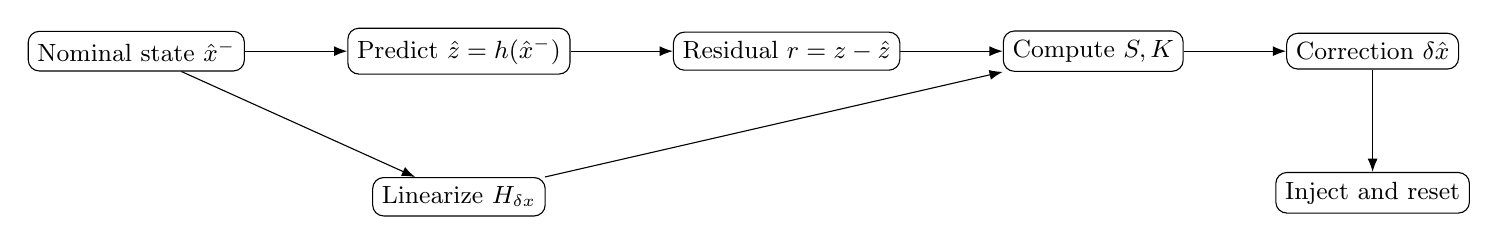
\begin{tikzpicture}[node distance=1.3cm,>=Latex, every node/.style={font=\small}]
\node[draw,rounded corners] (nom) {Nominal state $\hat x^-$};
\node[draw,rounded corners,right=of nom] (pred) {Predict $\hat z=h(\hat x^-)$};
\node[draw,rounded corners,right=of pred] (res) {Residual $r=z-\hat z$};
\node[draw,rounded corners,below=of pred] (lin) {Linearize $H_{\delta x}$};
\node[draw,rounded corners,right=of res] (gain) {Compute $S,K$};
\node[draw,rounded corners,right=of gain] (corr) {Correction $\delta\hat x$};
\node[draw,rounded corners,below=of corr] (inj) {Inject and reset};
\draw[->] (nom)--(pred); \draw[->] (pred)--(res); \draw[->] (res)--(gain); \draw[->] (gain)--(corr); \draw[->] (corr)--(inj); \draw[->] (lin)--(gain); \draw[->] (nom)--(lin);
\end{tikzpicture}
\end{center}

\subsection{Attitude Partials}
Suppose a measurement depends on a vector $\mathbf{a}^e=\Cbe\mathbf{a}^b$. With the attitude perturbation convention
\begin{equation}
\Cbe\approx(\I-\skew{\delta\boldsymbol\theta})\hat{\Cbe},
\end{equation}
then
\begin{align}
\mathbf{a}^e
&\approx(\I-\skew{\delta\boldsymbol\theta})\hat{\Cbe}\mathbf{a}^b\\
&=\hat{\mathbf{a}}^e-\skew{\delta\boldsymbol\theta}\hat{\mathbf{a}}^e\\
&=\hat{\mathbf{a}}^e+\skew{\hat{\mathbf{a}}^e}\delta\boldsymbol\theta.
\end{align}
Therefore,
\begin{equation}
\frac{\partial \mathbf{a}^e}{\partial\delta\boldsymbol\theta}=\skew{\hat{\mathbf{a}}^e}.
\label{eq:attitude_partial_vector_e_rev2}
\end{equation}
If the opposite attitude convention is used, the sign flips. This is one of the most common sign mistakes in ES-EKF measurement models.

\section{Generic Sensor Lever-Arm Model}
For sensor $s$ mounted at lever arm $l_{os}^b$, predicted sensor position and velocity are
\begin{align}
\hat{\rb}_s^e &= \hat{\rb}_{eo}^e+\hat{\Cbe}l_{os}^b,\\
\hat{\vb}_s^e &= \hat{\vb}_{eo}^e+\hat{\Cbe}\left(\hat{\boldsymbol\omega}_{eb}^b\times l_{os}^b\right).
\end{align}
The first-order position perturbation is
\begin{equation}
\delta\rb_s^e
=\delta\rb_{eo}^e+\frac{\partial(\Cbe l_{os}^b)}{\partial\delta\boldsymbol\theta}\delta\boldsymbol\theta+\hat{\Cbe}\delta l_{os}^b.
\end{equation}
Using \cref{eq:attitude_partial_vector_e_rev2},
\begin{equation}
\delta\rb_s^e
=\delta\rb_{eo}^e+\skew{\hat{\Cbe}l_{os}^b}\delta\boldsymbol\theta+\hat{\Cbe}\delta l_{os}^b.
\label{eq:sensor_pos_error_lever_rev2}
\end{equation}
Thus a position-like sensor with lever arm has attitude sensitivity even if its basic measurement is position.

\section{Loosely Coupled GNSS and INS}
For a GNSS antenna at lever arm $l_{og}^b$, the predicted antenna position is
\begin{equation}
\hat{\rb}_g^e=\hat{\rb}_{eo}^e+\hat{\Cbe}l_{og}^b.
\end{equation}
A loosely coupled GNSS position update has residual
\begin{equation}
\mathbf{r}_p=\mathbf{z}_{p,gps}^e-\hat{\rb}_g^e.
\end{equation}
The error-state Jacobian blocks are
\begin{equation}
\mathbf{H}_{p}=\begin{bmatrix}
\I & \zero & \skew{\hat{\Cbe}l_{og}^b} & \zero & \cdots & \hat{\Cbe}
\end{bmatrix},
\end{equation}
where the final block appears only if GNSS antenna lever-arm error is estimated.

For GNSS velocity, the predicted antenna velocity is
\begin{equation}
\hat{\vb}_g^e=\hat{\vb}_{eo}^e+\hat{\Cbe}\left(\hat{\boldsymbol\omega}_{eb}^b\times l_{og}^b\right).
\end{equation}
The velocity update residual is
\begin{equation}
\mathbf{r}_v=\mathbf{z}_{v,gps}^e-\hat{\vb}_g^e.
\end{equation}
The Jacobian includes direct velocity sensitivity, attitude sensitivity through the rotated lever-arm velocity term, gyro-error sensitivity through $\hat{\boldsymbol\omega}_{eb}^b$, and optional lever-arm sensitivity. In many systems the lever-arm velocity term is small, but for high angular-rate vehicles it can be essential.

\section{Tightly Coupled GNSS and INS}
For satellite $j$ at position $\rb_j^e$, receiver antenna position $\rb_g^e$, geometric range is
\begin{equation}
\rho_j=\norm{\rb_g^e-\rb_j^e}.
\end{equation}
The predicted pseudorange is
\begin{equation}
\hat z_{\rho,j}=\rho_j+c\hat b_c+\text{corrections},
\end{equation}
where $b_c$ may be in seconds or meters depending on convention. Define the line-of-sight unit vector from satellite to receiver as
\begin{equation}
\mathbf{u}_j^e=\frac{\rb_g^e-\rb_j^e}{\rho_j}.
\end{equation}
Then
\begin{equation}
\frac{\partial \rho_j}{\partial \rb_g^e}=\mathbf{u}_j^{eT}.
\end{equation}
Using \cref{eq:sensor_pos_error_lever_rev2}, the pseudorange Jacobian contains
\begin{equation}
\mathbf{H}_{\rho,j}=\begin{bmatrix}
\mathbf{u}_j^{eT} & \zero & \mathbf{u}_j^{eT}\skew{\hat{\Cbe}l_{og}^b} & \cdots & c & 0
\end{bmatrix}.
\end{equation}
Doppler or pseudorange-rate uses relative velocity projected along line of sight:
\begin{equation}
\dot\rho_j\approx \mathbf{u}_j^{eT}\left(\vb_g^e-\vb_j^e\right),
\end{equation}
with receiver clock drift entering additively. Carrier phase adds an ambiguity state and has similar geometry to pseudorange but with carrier wavelength scaling \cite{groves2013,kaplan2017,grewal2020}.

\section{Altimeter}
A barometric or radar altimeter generally measures height above a reference surface. Let altitude be represented by a scalar function $h(\rb_s^e)$ evaluated at the altimeter measurement point
\begin{equation}
\rb_s^e=\rb_{eo}^e+\Cbe l_{os}^b.
\end{equation}
A simple biased and scaled measurement model is
\begin{equation}
 z_{alt}=(1+s_{alt})h(\rb_s^e)+b_{alt}+v.
\end{equation}
The position sensitivity is
\begin{equation}
\mathbf{h}_r=\left.\frac{\partial h}{\partial\rb^e}\right|_{\hat{\rb}_s^e}.
\end{equation}
The error-state Jacobian includes
\begin{equation}
\mathbf{H}_{alt}=\begin{bmatrix}
(1+\bar s_{alt})\mathbf{h}_r & \zero & (1+\bar s_{alt})\mathbf{h}_r\skew{\hat{\Cbe}l_{os}^b} & \cdots & 1 & h(\hat{\rb}_s^e)
\end{bmatrix},
\end{equation}
where the final two columns correspond to altimeter bias and scale-factor states if estimated.

\section{Body-Frame Speed Sensor}
Suppose a speed sensor measures the body-forward component of velocity at sensor point $s$, after mounting rotation. Let $\mathbf{e}_x^s=[1,0,0]^T$ and let $\mathbf{C}_b^s$ map body components into sensor components. The predicted scalar measurement is
\begin{equation}
\hat z=(1+s_v)\mathbf{e}_x^{sT}\mathbf{C}_b^s\mathbf{C}_e^b\hat{\vb}_s^e+b_v.
\end{equation}
where
\begin{equation}
\hat{\vb}_s^e=\hat{\vb}_{eo}^e+\hat{\Cbe}(\hat{\boldsymbol\omega}_{eb}^b\times l_{os}^b).
\end{equation}
The direct velocity partial is
\begin{equation}
\frac{\partial z}{\partial\delta\vb^e}=(1+s_v)\mathbf{e}_x^{sT}\mathbf{C}_b^s\mathbf{C}_e^b.
\end{equation}
The attitude partial has contributions from rotating ECEF velocity into body and from the lever-arm velocity. In interview settings, the key point is that body-frame speed is not just a velocity measurement. It is attitude-coupled, mounting-coupled, and lever-arm-coupled.

\section{Magnetometer}
A magnetometer predicts the local magnetic field vector in the sensor frame:
\begin{equation}
\hat{\mathbf{z}}_m=\mathbf{C}_b^m\mathbf{C}_e^b\mathbf{m}^e(\hat{\rb}_s^e)+\bb_m.
\end{equation}
Lever arm usually matters weakly because Earth's magnetic field changes slowly over vehicle dimensions, but mounting misalignment, hard iron, soft iron, and local magnetic disturbances dominate the error model. Magnetometers can aid heading, but their integrity depends strongly on environment.

\section{Vision and Relative Navigation}
A camera measurement depends on sensor pose:
\begin{align}
\rb_c^e &= \rb_{eo}^e+\Cbe l_{oc}^b,\\
\mathbf{C}_e^c &= \mathbf{C}_b^c\Ceb.
\end{align}
For a landmark at $\rb_L^e$, the relative vector in camera coordinates is
\begin{equation}
\boldsymbol\rho_L^c=\mathbf{C}_e^c(\rb_L^e-\rb_c^e).
\end{equation}
A pinhole camera produces normalized image coordinates
\begin{equation}
\mathbf{z}=\begin{bmatrix}\rho_x^c/\rho_z^c\\\rho_y^c/\rho_z^c\end{bmatrix}+\mathbf{v}.
\end{equation}
The measurement Jacobian combines projection partials, relative-position partials, attitude partials, and lever-arm partials. This is the natural extension of the same lever-arm framework used for GNSS and air-data sensors.

\chapter{Latency, Asynchronous Measurements, and Smoothing}
\section{Multi-Rate Navigation Systems}
Placeholder.
\section{Out-of-Sequence Measurements}
Placeholder.
\section{State History Buffering}
Placeholder.
\section{Rewind-Replay Architectures}
Placeholder.
\section{Fixed-Lag Smoothing}
Placeholder.
\section{Rauch-Tung-Striebel Smoothing}
Placeholder.
\section{Real-Time Tradeoffs}
Placeholder.

\chapter{Filter Consistency, Validation, and Tuning}
\section{Innovation Residuals}
Placeholder.
\section{Innovation Covariance}
Placeholder.
\section{Normalized Innovation Squared}
Placeholder.
\section{Normalized Estimation Error Squared}
Placeholder.
\section{Covariance Realism}
Placeholder.
\section{Process Noise Tuning}
Placeholder.
\section{Measurement Noise Tuning}
Placeholder.

\chapter{Observability}
\section{Formal Observability Theory}
Placeholder.
\section{INS and GNSS Observability}
Placeholder.
\section{Bias Observability}
Placeholder.
\section{Scale-Factor Observability}
Placeholder.
\section{Misalignment Observability}
Placeholder.
\section{Trajectory-Dependent Observability}
Placeholder.
\section{Practical Examples}
Placeholder.

\chapter{GPS Integrity, Resilience, and Alternative PNT}
\section{RAIM}
Placeholder.
\section{ARAIM}
Placeholder.
\section{Chi-Square Fault Detection}
Placeholder.
\section{CRPA}
Placeholder.
\section{DIGAR}
Placeholder.
\section{M-Code}
Placeholder.
\section{Anti-Jam and Anti-Spoofing}
Placeholder.
\section{Iridium PNT Concepts}
Placeholder.
\section{Signals of Opportunity}
Placeholder.
\section{GPS-Denied Navigation}
Placeholder.

\chapter{Advanced Navigation Topics}
\section{Transfer Alignment}
Placeholder.
\section{Gyrocompassing}
Placeholder.
\section{Calibration}
Placeholder.
\section{Factor Graph Optimization}
Placeholder.
\section{Navigation Trade Studies}
Placeholder.

\chapter{Embedded Navigation Software and Modern C++}
\section{Real-Time Navigation Software Design}
Placeholder.
\section{Sensor Interface Architectures}
Placeholder.
\section{Memory and Performance Considerations}
Placeholder.
\section{Templates and Static Polymorphism}
Placeholder.
\section{Dynamic Polymorphism}
Placeholder.
\section{Smart Pointers}
Placeholder.
\section{STL Containers}
Placeholder.
\section{Modern C++ Features}
Placeholder.
\section{Navigation Software Design Patterns}
Placeholder.

\backmatter
\printbibliography
\end{document}
